\documentclass[10pt,twocolumn,letterpaper]{article}

\usepackage{cvpr}
\usepackage{times}
\usepackage{epsfig}
\usepackage{graphicx}
\usepackage{amsmath}
\usepackage{amssymb}
\usepackage{fancyvrb}

% Include other packages here, before hyperref.

% If you comment hyperref and then uncomment it, you should delete
% egpaper.aux before re-running latex.  (Or just hit 'q' on the first latex
% run, let it finish, and you should be clear).
\usepackage[breaklinks=true,bookmarks=false]{hyperref}

\cvprfinalcopy % *** Uncomment this line for the final submission

\def\cvprPaperID{****} % *** Enter the CVPR Paper ID here
\def\httilde{\mbox{\tt\raisebox{-.5ex}{\symbol{126}}}}

% Pages are numbered in submission mode, and unnumbered in camera-ready
%\ifcvprfinal\pagestyle{empty}\fi
\setcounter{page}{1}
\begin{document}
	
	%%%%%%%%% TITLE
	\title{Neural fiber tractography with Diffusion Tensor Imaging(DTI) and Deep Learning}
	
	\author{Yixuan Tan, Zhicheng Gu\\
		University of Wisconsin - Madison\\
		{\tt\small ytan39@wisc.edu, zgu58@wisc.edu}
		% For a paper whose authors are all at the same institution,
		% omit the following lines up until the closing ``}''.
		% Additional authors and addresses can be added with ``\and'',
		% just like the second author.
		% To save space, use either the email address or home page, not both
		%\and
		%Zhicheng Gu\\
		%University of Wisconsin - Madison\\
		%{\tt\small zgu58@wisc.edu}
	}
	
	\maketitle
	%\thispagestyle{empty}
	
	%%%%%%%%% ABSTRACT
	\begin{abstract}
		In-vivo neural fiber detection can be very useful for studying brain functionalities. With data gathered by diffusion tensor MRI (DTI), people used to perform tractography by tracing single fiber bundle starting from seed points whose performance depends strongly on the choice of seeds. In our project, we overcame this drawback by adopting deep learning network as the new tractography algorithm. We successfully trained our network to predict if a voxel is on neural fiber or not. We also disscussed advantages, disvantages and possible improvements for this DNN-based model.
	\end{abstract}
	
	%%%%%%%%% BODY TEXT
	\section{Introduction}
	
	Anatomic study of spatial distribution of neural fiber bundles and their connections in human brains has played an important role in studies of brain functions including brain diseases, neural science, psychology etc. However, with more and more complicated situations being studied, the requirement of measurement being noninvasive and in-vivo becomes non-negligible. As the first and mostly used noninvasive, in-vivo imaging modality with the potential to generate fiber-tract trajectories in soft fibrous tissues, Diffusion tensor MRI (DTI) was first adopted for use in clinical neuroradiology during the early 1990s~\cite{mukherjee2008diffusion}. Its non-invasive nature and ease of whole-brain simultaneous measurement makes it possible to compare areal connections in humans across many cortical and subcortical sites. Furthermore, real-time results can be combined with other real-time in-vivo measures to reveal interconnections between neuron activities and human behavior across individuals~\cite{humanconnectblog}.
	
	One important aspect of studying DTI involves optimizing tractography algorithms to maximize accuracy and minimize errors in the diffusion tractography data. Diffusion is the spread of molecules in a fluid due to constant thermal motion. The extent of this spread depends on the diffusivity of the medium. In soft fibrous tissues such as brain white matter, diffusion is slower across than along such fibers. Hence, by measuring diffusion along many directions and observing that it is faster in one direction than in others, we can deduce the direction of the fiber bundles at every point in the brain. Traditional DTI fiber tracking algorithms can be divided into deterministic and probabilistic methods, both requires manually added seed voxels to start from and traces down a (probabilistic) voxel pathway along the direction of maximum diffusion speed. Some of the main drawbacks in traditional methods include~\cite{basser2000vivo}: 1. Seed: accuracy has a large dependence on choice seeds; 2. Nearsightedness: identification of fiber based solely on change of major diffusion direction in adjacent voxels; 3. Crossing: hard to trace in regions where fibers cross and merge into each other.
	
	In this project, we tried to solve these drawbacks by using a deep learning neural network (DNN). We implemented and trained our DNN to perform tractography over the whole brain. Specifically, we tried to do two things: 1. classify if each voxel is on neural fiber or not and 2. output direction of neural fiber for voxels on neural fiber. The first task was successfully completed while the second was still in working. In this report, we will first introduce the implementation of the DNN-based tractographer (part 2 and 3) and its performance (part 4). Then we will discuss its advantages and disadvantages as compared with traditional methods (part 5), and diffficulties we encountered in doing this project.
	
	%-------------------------------------------------------------------------
	\section{Data Proprocessing}
	
	\subsection{Raw MRI Data}
	
	The raw MRI data we used was from the Human Connectome Project (HCP) led by Washington University in Saint Louis, University of Minnesota and Oxford University. They provided publicly downloadable data at their CONNECTOME-DB~\cite{humanconnect}. The data we used was from the "diffusion preprocessed" dataset under "WU-Minn HCP Data - 900 Subjects + 7T". For this project, we downloaded only 10 uncorrelated subjects and used only 4 of them for training/testing.
	
	\subsection{Synthesizing to DTI using Camino}
	In order to calculate a DTI image from the downloaded raw MRI data (each subject contains 200+ MRI images taken from different angles), we used the camino~\cite{cook2006camino} library from UCL.
	(Files in bold font are original data in HCP's archive)
	\begin{enumerate}
\item 
Generate a scheme file that stores information of gradient correction of each MRI image, data used were in downloaded package(bvecs and bvals):
\begin{Verbatim}[commandchars=\\\{\}]
$ fsl2scheme -bvecfile \textbf{bvecs} 
-bvalfile \textbf{bvals} > hcp.scheme
\end{Verbatim}


\item
Convert raw data in NIfTI data format to camino’s own format .Bfloat:
\begin{Verbatim}[commandchars=\\\{\}]
$ image2voxel -4dimage \textbf{data.nii.gz} 
-outputfile dwi.Bfloat
\end{Verbatim}


\item
Fit diffusion tensor from raw data:
\begin{Verbatim}[commandchars=\\\{\}]
$ modelfit -inputfile dwi.Bfloat 
-schemefile hcp.scheme -gradadj 
\textbf{grad_dev.nii.gz} -model ldt -bgmask 
\textbf{nodif_brain_mask.nii} -outputfile 
dt.Bdouble
\end{Verbatim}


\item
Convert the output back to NIfTI format so we can read it to generate feature vector to feed in our NN:
\begin{Verbatim}[commandchars=\\\{\}]
$ dt2nii -inputfile dt.Bdouble 
-outputroot nifti_ 
-header \textbf{data.nii.gz}
\end{Verbatim}


\item
Also, for future visualization purposes, compute fractional anisotropy graph:

\begin{Verbatim}[commandchars=\\\{\}]
$ for PROG in fa md; do
$ cat dt.Bdouble | ${PROG} | 
voxel2image -outputroot 
${PROG} -header \textbf{data.nii.gz}
$ done
\end{Verbatim}



	\end{enumerate}
	
	
	\subsection{Seed}
	To obtain label/ground truth, we need to apply traditional tractography algorithm on DTI image above. To do that, we need to first manually seed the DTI image. We used the ITK snap~\cite{yushkevich2006user} tool to open the original data.nii file, which displays it as a figure. We then put some seeds in the figure and save the seeds in a file called cc.nii.gz.
	
	\subsection{Tract fibers}
	Then we go back to camino and use the track tool with default parameters to perform tractography:
	
	\begin{verbatim}
	$ track -inputmodel dt -seedfile 
	cc.nii.gz -anisthresh 0.2 
	-curvethresh 60 -inputfile 
	dt.Bdouble > CCtracts.Bfloat
	\end{verbatim}
	
	In order to be able to read and visualize our ground truth, we need to convert it to some general file format, we choose to convert to .vtk as follows:
	
	\begin{verbatim}
	$ vtkstreamlines -colourorient 
	< CCtracts.Bfloat > CCtracts.vtk
	\end{verbatim}
	
	
	Then we used Paraview~\cite{ayachit2015paraview} to look at the tracts and save it as a .csv file which we will read and use to generate labels.
	
	\subsection{Data Generation}
	With synthesized DTI image file and traced tracts file, we wrote a piece of matlab code to generate the training and test data. This piece of code can perform three tasks:
	
	\begin{enumerate}
		\item
		Form the traced tract file, read all points. Round their coordinates to integer to represent voxel position. From the DTI image, pick these points and store their diffusion tensor data (of 5*5*5 vicinity) and label it as on fiber (label = 1).
		
		\item
		From DTI data, sparsely sample equally spaced voxels and store same information as in 1). Note here the label is stored as the actual label, but since the on-fiber voxels are very few and compact distributed, there is little overlap between data in 2.5.1 and 2.5.2.
		
		\item
		Store same structured data (w/o label) for all voxels in a DTI image. 
	\end{enumerate}
	
	We use 2.5.1 and 2.5.2 to generate training data and 2.5.3 to generate test data to perform DNN-based tractography over the whole brain on.
	
	
	%-------------------------------------------------------------------------
	
	\section{Deep Learning Network}
	
	\subsection{Framework}
	
	We use Tensorflow~\cite{tensorflow} as the computing system. TensorFlow is an open source software library provided by Google. It does numerical computation using data flow graphs. 
	
	We use Keras~\cite{keras} to build the deep learning model. Keras is a high-level neural networks library, which is running on the  TensorFlow or Theano. We choose TensorFlow because it is more famous and easy to install and use. Keras is wriiten in Python, and enables fast building and experimentation. This great feature saves us a lot of time and energy.
	
	\begin{figure*}[!htbp]
		\begin{center}
			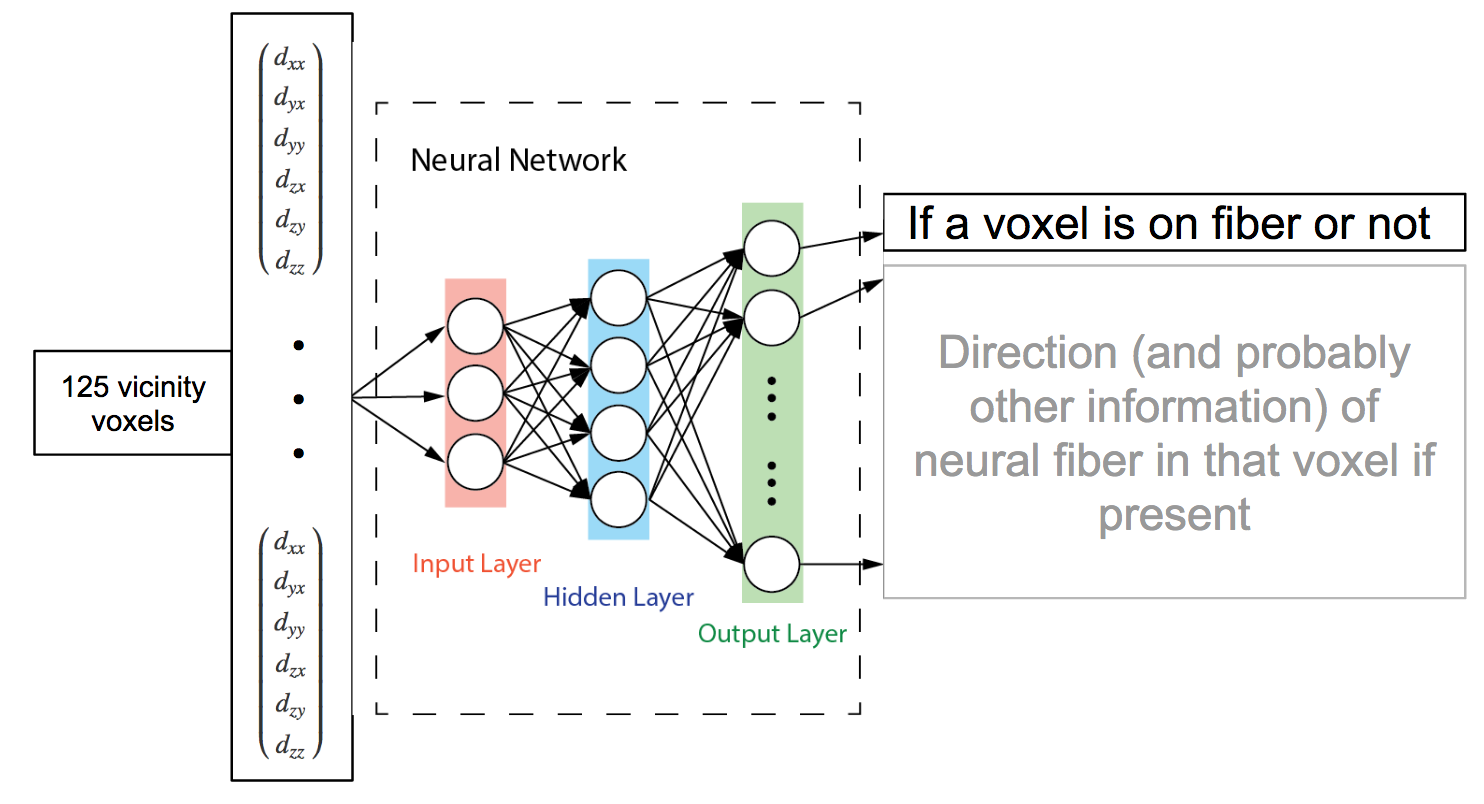
\includegraphics[width=0.9\linewidth]{img/6.png}
		\end{center}
		\caption{Deep learning network structure.}
		\label{fig:network}
	\end{figure*}
	
	\subsection{Network Structure}
	
	We cut the entire figures into 5*5*5 blocks. Each voxels will be at the center of one block. The tensor values of all of the neighbors in this 5*5*5 block is used to predict the feature of the center voxel. The network structure is shown in Figure~\ref{fig:network}.
	
	We use a fully connected neural network to train the data. The detail of the network is described below. We also consider using the convolutional neural network for this task, but the convolutional neural network in 3D space is hard to implement. Also, the data we are using has 6 parameters at each voxel, which makes it even harder to implement the convolutional neural network.
	
	\begin{itemize}
		\item Input Layer. 
		
		The input layer of the network has 750 dimensions, which is equal to 6 (number of tensor parameters at each voxel) * 5 (length) * 5 (width) * 5 (height) = 750 features dimensions. Each feature is a float number. The original number is really small, which is around 1E-10 to 1E-15. We scale the features to about -10.0 to 10.0.
		
		\item Hidden Layer
		
		We try different structures of hidden layers, such as ~\cite{deepbig}. We find that increasing number of hidden layers does not increase the final result. Two hidden layers already gives out the best result we can get. Also, when the neurals in each hidden layers is more than 2000, the result does not increase any more. Hence, the final structure we are using has two hidden layers, each has 2048 neurals.
		
		\item Output Layer
		
		Currently, the output has only dimension, which means if this voxel is on fiber or not. In general, we also want to get the direction of each points on the fibers. This requires the network has multidimensional output. Due to the time limit we couldn't finish this part, but the current result is good enough to find all of the voxels on the fibers.
		
	\end{itemize}
	
	
	
	\subsection{Parameters}
	
	\begin{itemize}
		\item Activation Function
		
		We try the following three activation functions: \textit{relu}, \textit{sigmoid} and \textit{tanh}. The performance of \textit{relu} activation function is really bad. The outputs are all 1 or 0 because the network can't extract meaningful features from the training datas. The performance of \textit{sigmoid} and \textit{tanh} function is similar, and the \textit{sigmoid} function is a little better. So we choose \textit{sigmoid} activation function at the activation function of our network.
		
		\item Dropout
		
		Dropout in deep learning network is used to avoid overfitting. Our network should not have overfitting problem because our training time is relative short due to the resource constraint. Since this technique is always used in deep learning network, we still add a 0.5 dropout parameter to our network. The result of network with dropout is almost the same with the network without dropout.
		
		\item Loss Function
		
		Since the output is only one dimension, we use binary cross entropy as the loss function. This is the most widely used loss function for binary classification.
		
	\end{itemize}
	
	\subsection{Training}
	
	We set the training epoch to 20 and batch size to 32. It takes us about ten minutes to training the network with training data from one MRI figure, and it takes more time to train the network with data from four MRI figures. Each MRI figure has more than one million voxels and the file size after processing is larger than 1 GB. Due to the time and resource limit we can't train our network on a larger dataset. The test result does not increase significantly after 10 epochs training. 
	
	
	\section{Result}
	
	\subsection{Prediction Demonstration}
	Results of an actual prediction using DNN of fiber location in an unseen brain is shown in Figure~\ref{fig:result1} and Figure~\ref{fig:result2}. The background of Figure~\ref{fig:result1} shows the fractional anisotropy (FA) of DTI image we used. It has brighter color where diffusion has higher anisotropy and darker color where diffusion is more isotropic. As a result, bright-colored region should be most fiber bundles rest. Compared with FA as well as with Figure~\ref{fig:streamline1} which is the result of traditional streamline method, it can be clearly seen that our method predicted if a voxel is on fiber or not correctly for most voxels.
	
	For a better view of this result, we attached .fig files in our submission so that you can drag and look at it from different directions.
	
	\begin{figure}[t]
		\begin{center}
			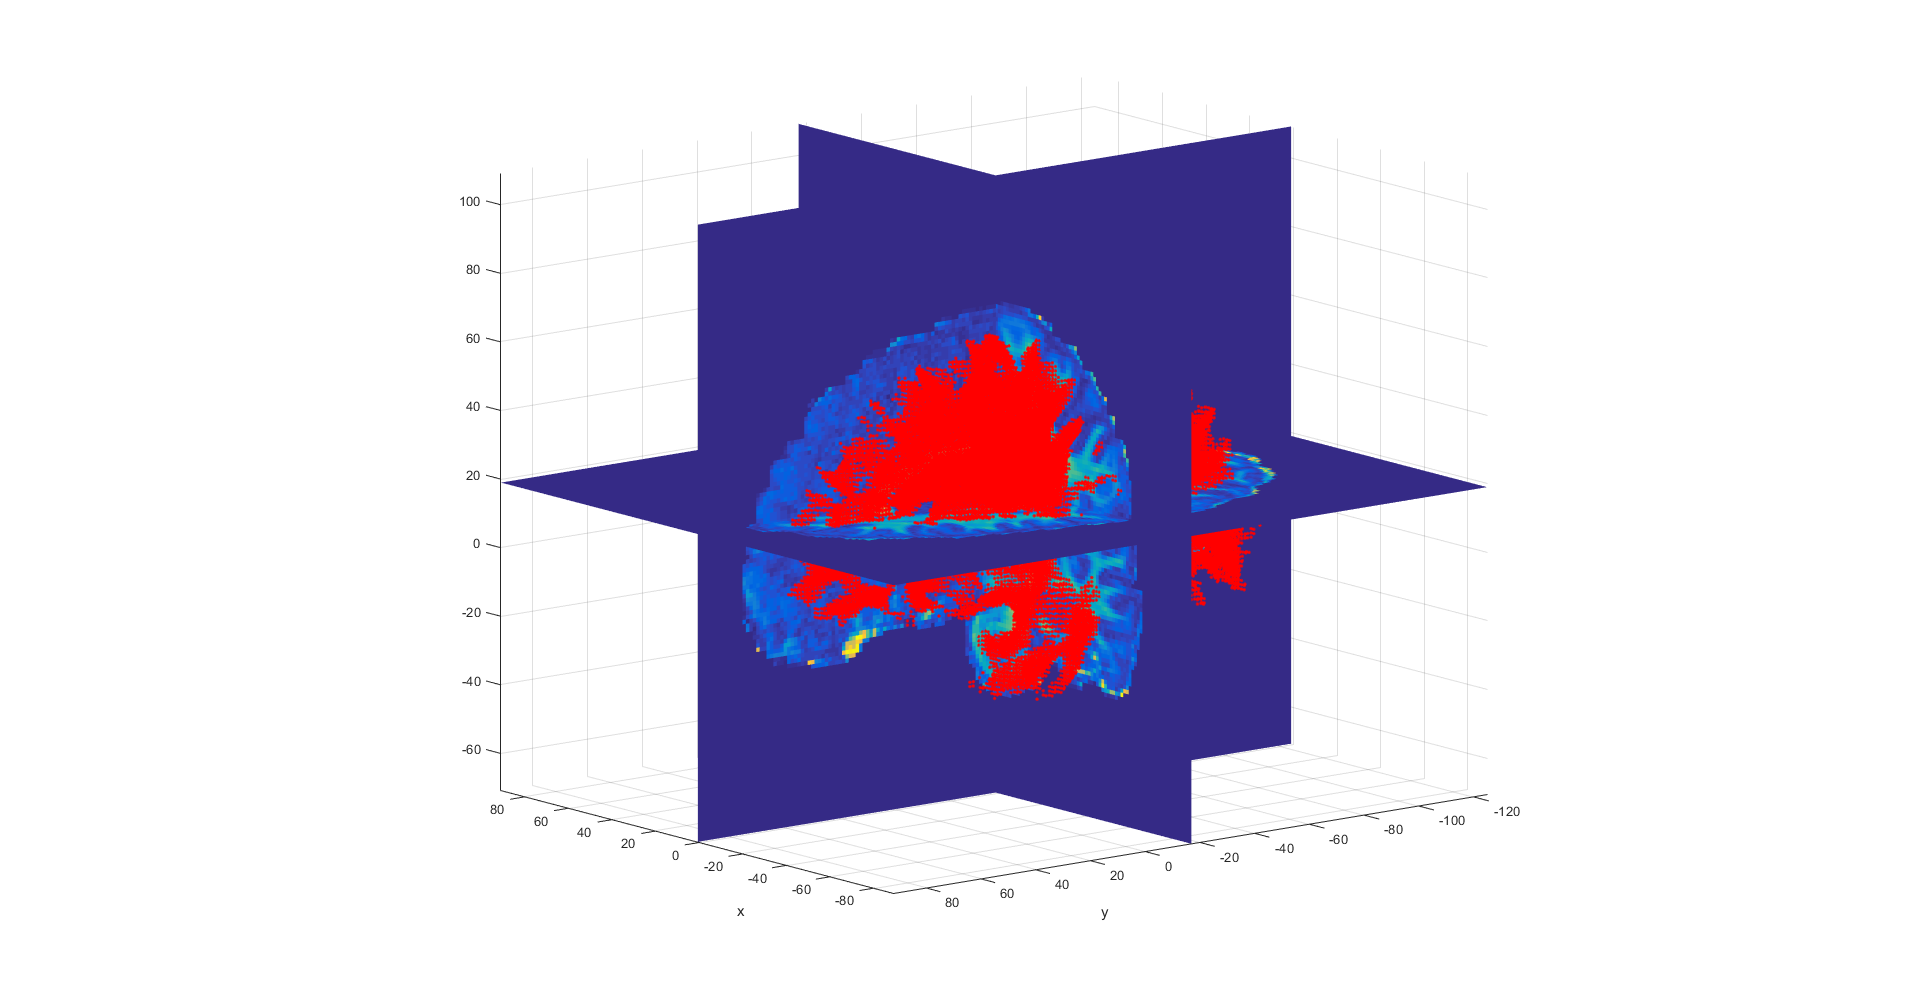
\includegraphics[width=1.0\linewidth]{img/1.png}
		\end{center}
		\caption{Result of deep learning training.}
		\label{fig:result1}
	\end{figure}
	
	\begin{figure}[t]
		\begin{center}
			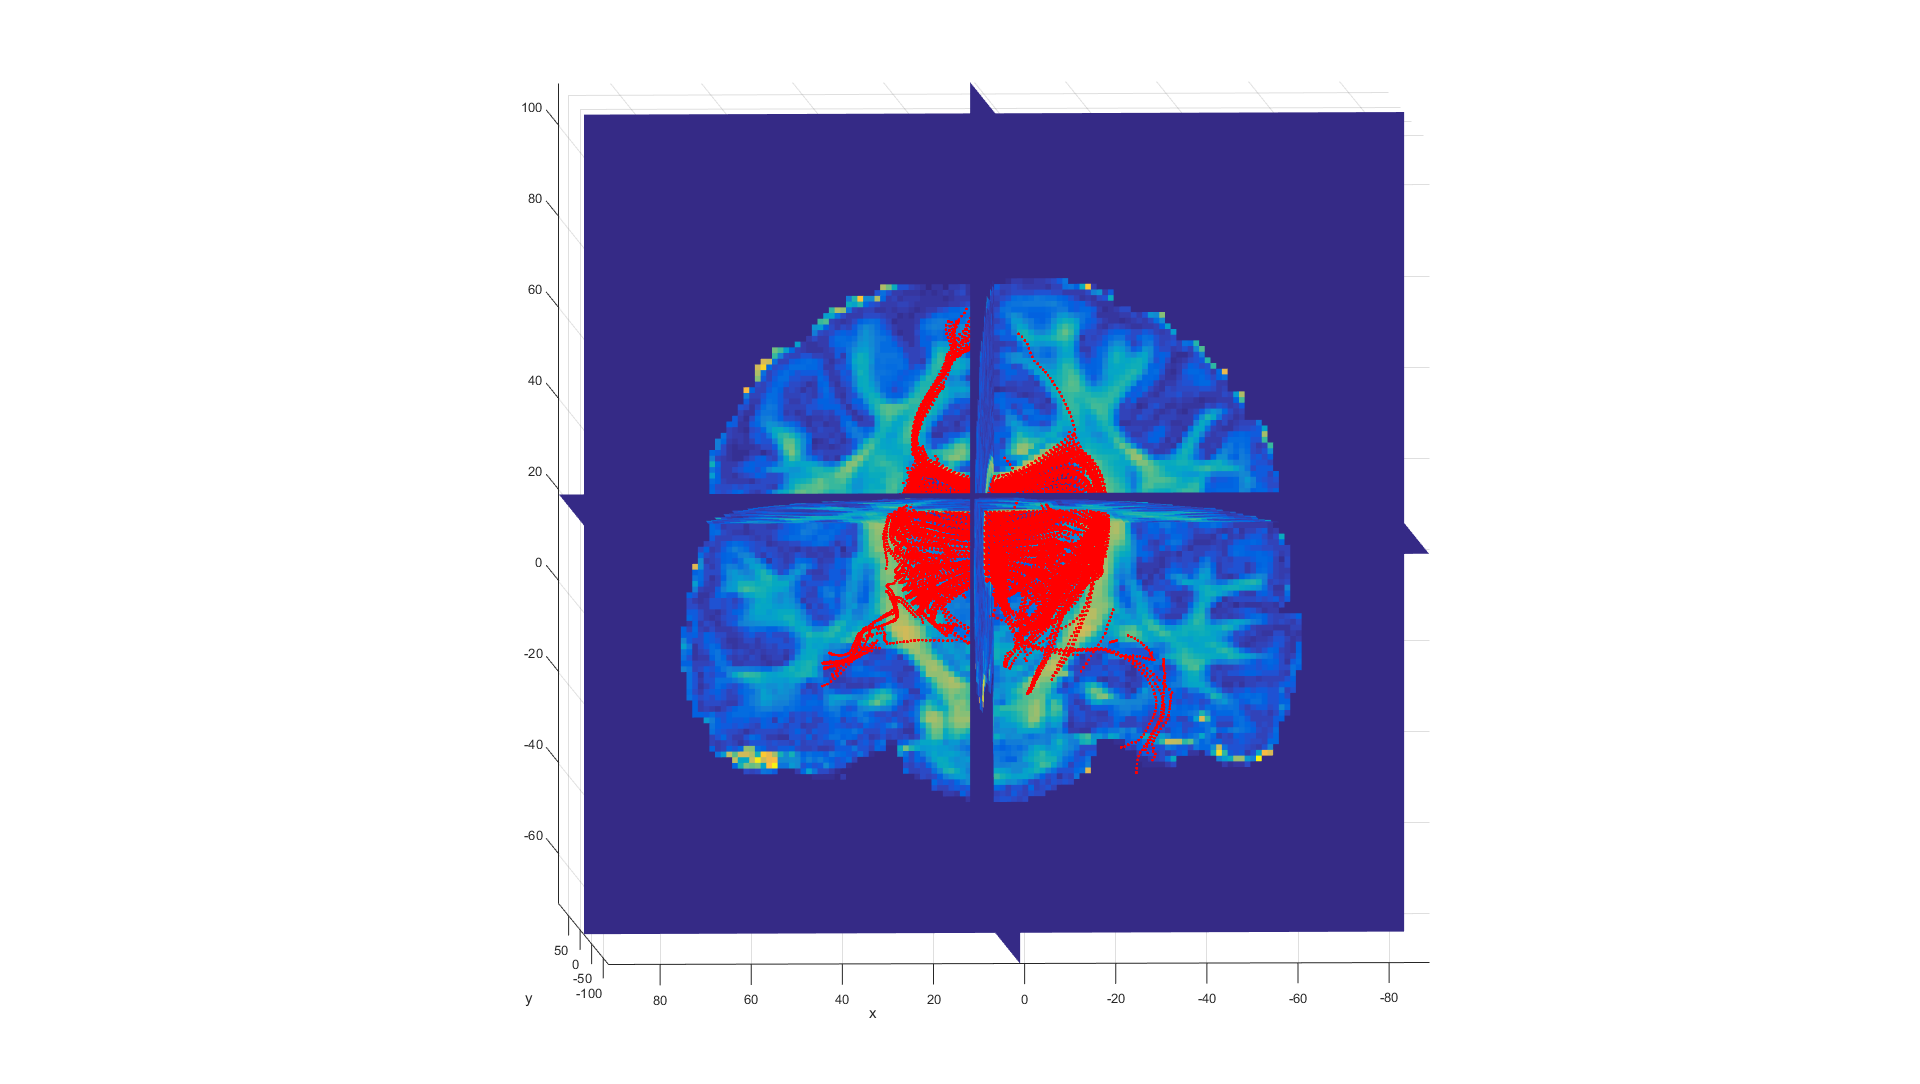
\includegraphics[width=1.0\linewidth]{img/5.png}
		\end{center}
		\caption{Result of traditional streamline algorithm with seed in the center.}
		\label{fig:streamline1}
	\end{figure}
	
	\begin{figure}[t]
		\begin{center}
			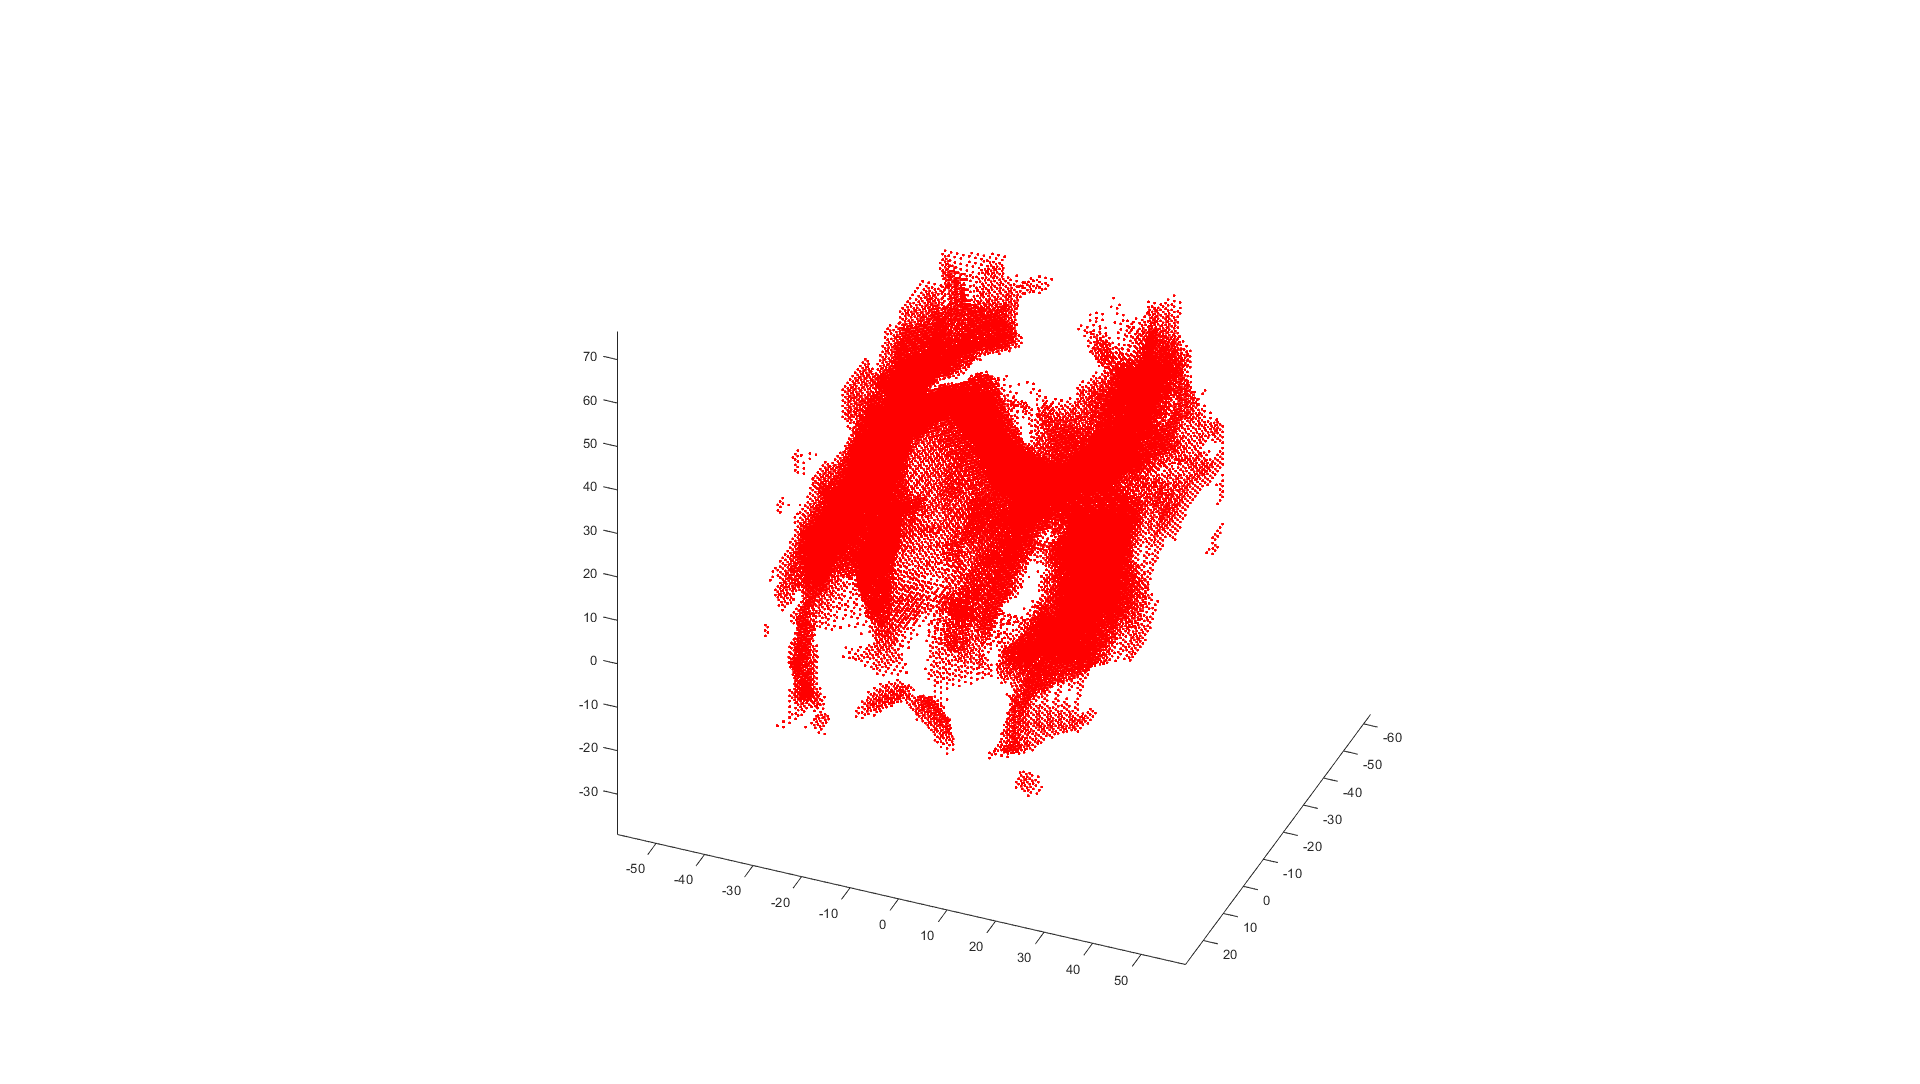
\includegraphics[width=1\linewidth]{img/2.png}
			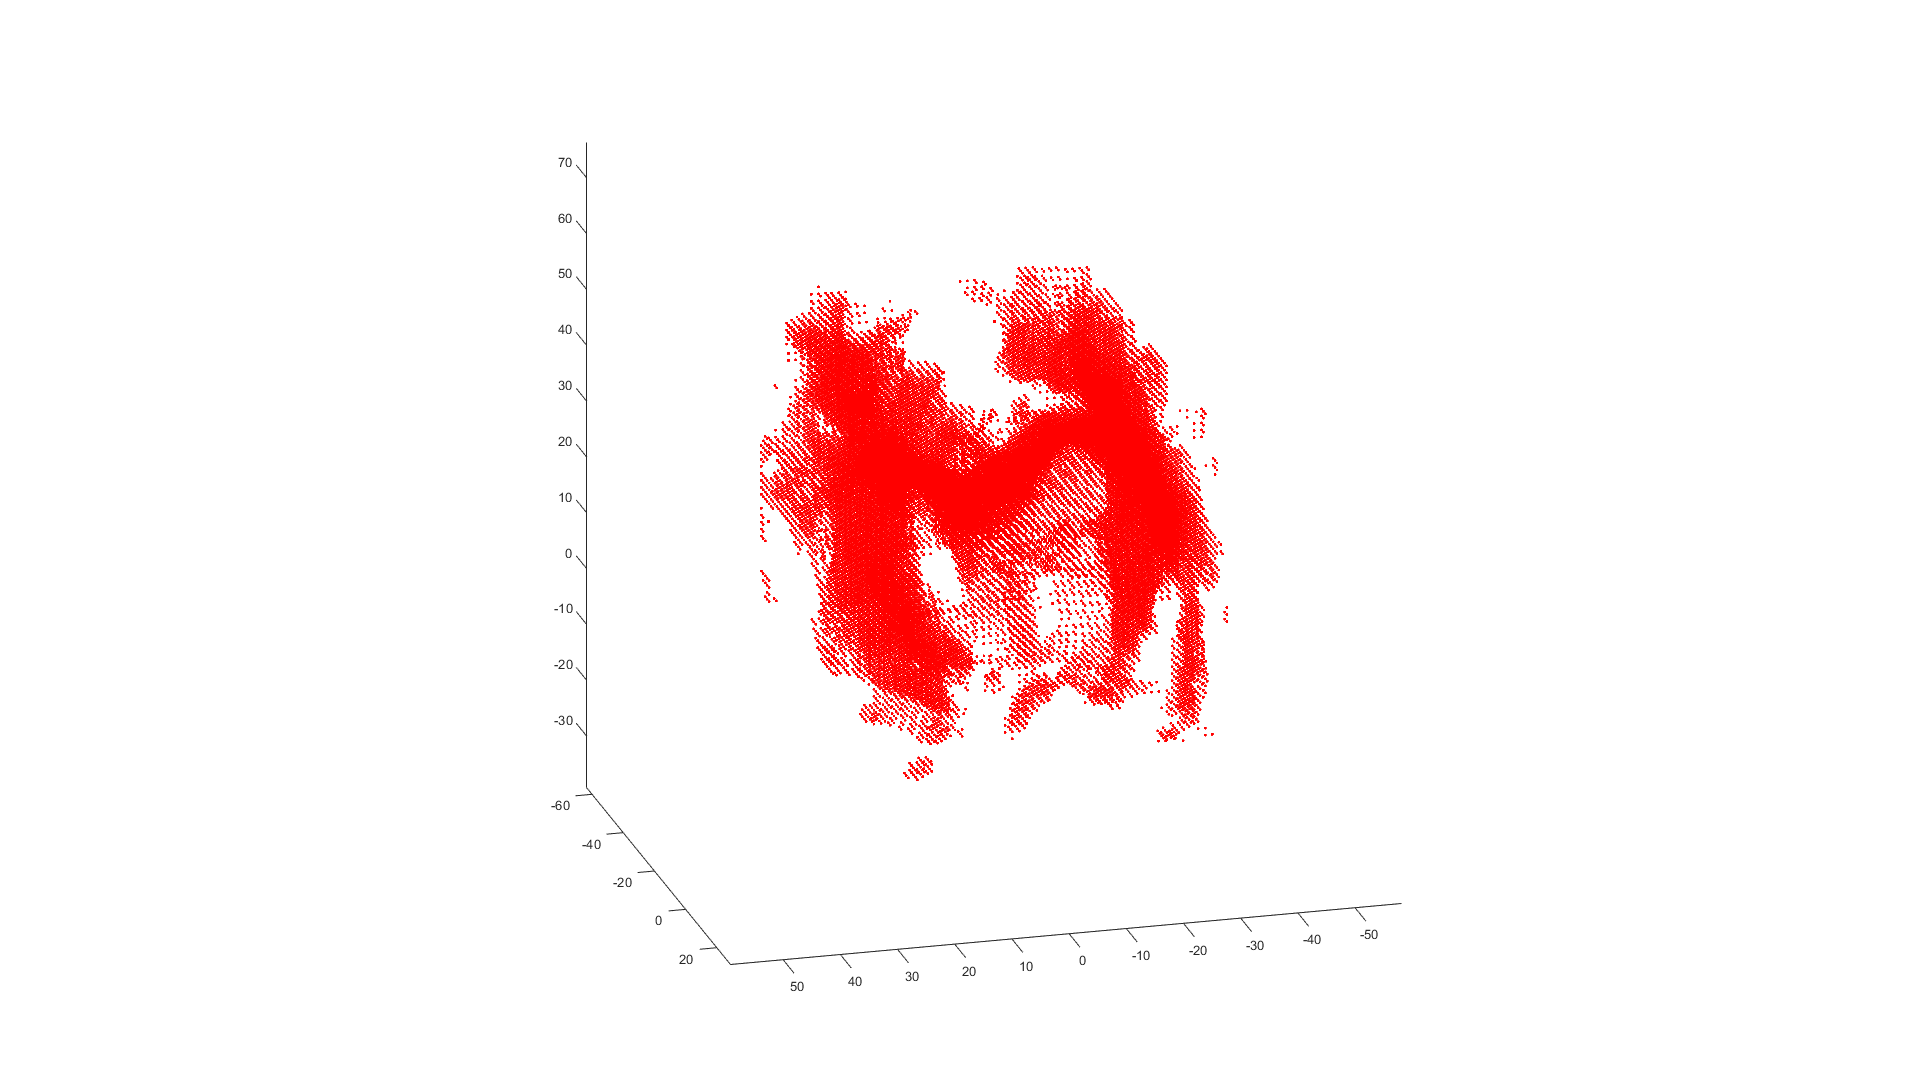
\includegraphics[width=1\linewidth]{img/3.png}
		\end{center}
		\caption{Result of deep learning training: a closer view.}
		\label{fig:result2}
	\end{figure}
	
	
	
	\subsection{Accuracy}
	The confusion matrix of our DNN is shown in Table~\ref{table1}. It shows the number of voxels of correct and incorect classifications. We need to emphasize that a high false positive rate (FPr) is not a big problem here because a high FPr could be because we identified on-fiber voxels not connected to seeds we used in traditional tractography method and therefore was not correctly marked in ground truth.
	
	\begin{table}[h]
		\begin{center}
			\begin{tabular}{|cc|c|c|}
				\hline
				& & \multicolumn{2}{c|}{Prediction} \\ \cline{3-4}
				& & 0 & 1\\
				\hline
				\multicolumn{1}{|c}{Truth} & \multicolumn{1}{|c|}{0} & 111419 & 30859\\ \cline{2-4}
				\multicolumn{1}{|c}{} & \multicolumn{1}{|c|}{1} & 7624 & 8798\\
				\hline
			\end{tabular}
		\end{center}
		\caption{Confusion Matrix}
		\label{table1}
	\end{table}
	
	
	\subsection{Learning Curve}
	The learning curve is shown in Figure~\ref{fig:learningcurve}. The test set prediction accuracy can reach 90\% with only 20000 training instances (voxels). Considering we have over 1 million voxels per DTI graph per brain, the efficiency of DNN in tiber tracking tasks is very high.
	
	\begin{figure}[t]
		\begin{center}
			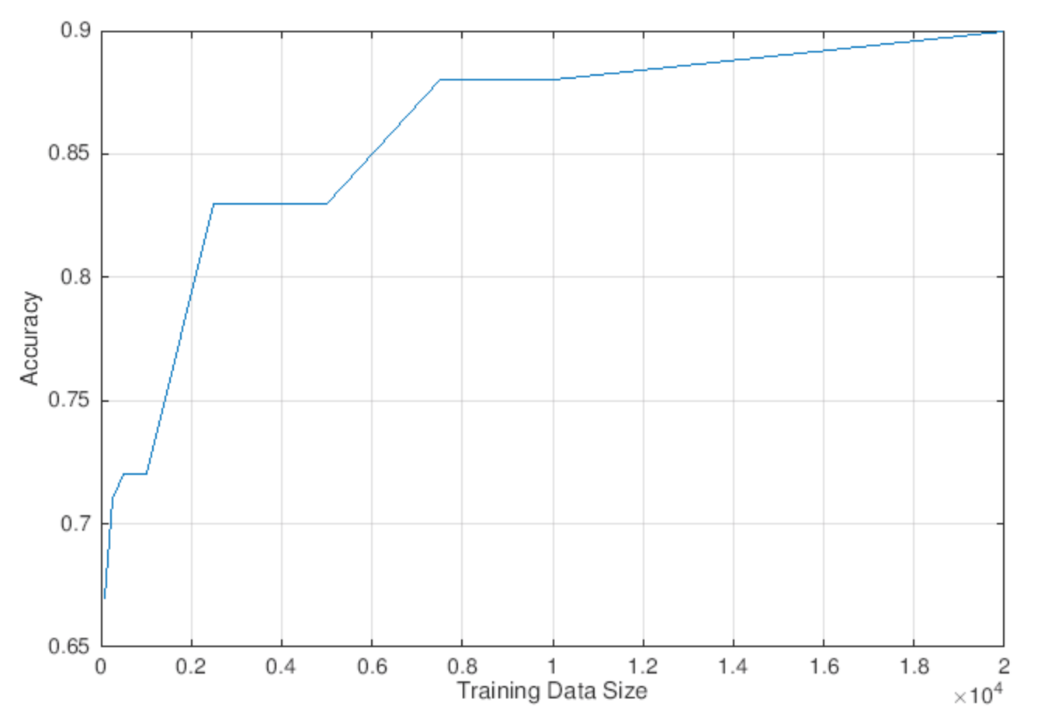
\includegraphics[width=0.8\linewidth]{img/8.png}
		\end{center}
		\caption{Learning Curve.}
		\label{fig:learningcurve}
	\end{figure}
	
	
	
	%-------------------------------------------------------------------------
	
	\section{Discussion}
	
	\subsection{Advantage of DNN}
	The advantage of using DNN-based tractography model lies in 3 parts:
	\begin{enumerate}
		\item 
		\textbf{Seed-Free}:
		As is obvious, DNN doesn’t require initial seeds to perform tractography which makes the algorithm more robust in two folds. On the one hand, this algorithm is operator independent making it stable and widens its potential usage. This means it's more reliable to compare results between different individuals or data acquired in different times. Although difference in DTI data acquisition persists, the effect of choice of different seeds among different samples will be eliminated.
		
		On the other hand, seed-free means increased accuracy because we can detect some on-fiber voxels which are not connected with seeds and thus can never be detected with seed-dependent algorithms. This can be clearly seen in our result Figure~\ref{fig:result1} and Figure~\ref{fig:streamline1}, neural fibers near brain surface are missed with traditional algorithm but correctly captured in our DNN-based model.
		
		\item
		\textbf{Real-time \& fully automatic}:
		With our DNN-based model, it’s possible to make outputting of neural fiber distribution from measured MRI data fully automatic. Also, since classification using a well trained DNN is very fast, the whole process could be made semi-real-time with bottleneck only at speed of MRI data acquisition. This could enable real-time, in-vivo visualization and analyzation of brain activity on an unprecedented neural fiber bundle level. This could benefit any study that involves characterizing neural reaction to external stimuli.
		
		
		\item
		\textbf{Convolutional neural network(CNN) with global information}:
		A DNN-based tractography model can be easily generalized to a CNN-based model. In our implementation, by picking only a 5*5*5 vicinity, we essentially performed the convolution step by hand. However, this implementation eliminated the possible mutual information from other parts of the brain. By generalizing to a real CNN, information from other parts of the brain could be combined into local information in later convolution layers, enabling us to use global brain information to classify each voxel which could add to the global accuracy.
		
	\end{enumerate}
	
	\subsection{Disadvantage of DNN}
	One major drawback for any voxel-based tractography model including DNN-based one, however, is that for non-voxel-aligned fibers and/or different fibers in adjacent voxels, it’s probable that these algorithms cannot differentiate between them. This can be solved by training the network to output, for each on-fiber voxel, the direction of its fiber and then apply some smoothing to voxels along that direction as postprocessing. If the goal for doing whole-brain neural tractography is only to identify connections between cortical regions, the direction of single fiber bundle can also be omitted.
	
	
	\section{Possible Improvements}
	
	\subsection{Fiber direction prediction}
	Right now we only predict whether a voxel is on fiber or not. We mark the voxel with 1 if the voxel is on the fiber and 0 if the voxel is not on the fiber. Although this method can show the entire distribution of the fibers, it is more like finding the white matters in the MRI figure. To get a more meaningful result, we also need the direction of the fibers at each voxels. The deep learning network need to be changed in order to get the direction of the fibers. We don't have enough time to do this because we already spend a lot of time on data processing and building the basic neural network. 
	
	
	\subsection{Optimize accuracy}
	The accuracy of our result can still be improved. To get a better result, we need to tune parameters of our system in a more precise way which usually costs a lot of time (see details in the difficulties part) and need good understanding of the deep learning algorithm. After tuning we can get a better result with less noisy points.
	
	Also, the feature vector can be changed. In this project we use six tensor values as in the original data. After doing some search we find that we can also get the direction features at each voxel. However, these features seems intuitive and we can't get more meaningful feature because the lack of domain knowledge.
	
	Furthermore, we can also modify the structure of deep learning network. Like we already mentioned, the convolutional neural network usually has a better performance than the fully connected network when the dataset is 2D figures. When it comes to 3D space, the convolutional or other similar methods might also have better performance than fully connected network. 
	
	\subsection{Try other labeling algorithm}
	The purpose of this project is to analysis the deep learning algorithm based tractography method. Different from traditional streamline methods, deep learning network needs a lot of training data. To get the label for training data, the only choice we have is to run a streamline algorithm (or some other traditional algorithm) and take the result as the label. Note that this is not the ground truth. If there is any error in the streamline algorithm, our deep learning network could also be influenced.
	
	To get a better ground truth label, we need to get the label from real world or by manual labeling. If we can get the label from real world, this is much easier. If not, we can also get the label by manually labeling. Considering the size of the data, this require a lot of work. Another approach is combian different traditional algorithms and get a labeling system with a higher accuracy. Then use this system to train the deep learning network.
	
	\subsection{Release of current work}
	Since we did make some progress, we could release our code to the community to help further the study. We already gathered all pieces of the code we used (including code for generating training/test data, code for NN and other supporting functions like result visualization) and put them together with some demostration results in the attachment. Furthermore, we need to wrap all of the codes and release them to the community. We hope this could be a useful resource for people who wants do a tractography with deep learning approach.
	
	
	\section{Difficulties in doing the project}
	The major difficulty we encountered was time vs amount of data. We planned to optimize our network a bit more or even to CNN, but then realized generating training data could take us 5 hours per training/test set (originally this can take longer than 1 day and we optimized our matlab code to get it down to 5 hours). Also, training and classifying over a desired amount of data (~ 20000 training instances for example) can take up to ~15 minutes per trial which slows down our pace.
	
	%-------------------------------------------------------------------------
	
	
	
	{\small
		\bibliographystyle{ieee}
		\bibliography{report}
	}
	
\end{document}
